\documentclass[10pt]{article}

%%%%%%%%%%%%%%%%%%%%%%%%%%%%%%%%%%%%%%%%%%%%%%%%%%%%%%%%%%%%%%%%%%%%%%%%%%%%%%%
%%% packages %%%
%%%%%%%%%%%%%%%%%%%%%%%%%%%%%%%%%%%%%%%%%%%%%%%%%%%%%%%%%%%%%%%%%%%%%%%%%%%%%%%

\usepackage[english]{babel} % Choose english language
\usepackage[labelfont = bf, font = small]{caption} % Use caption package. Use bold font for caption.
\usepackage{siunitx} % Use siunitx for unit representation.
\newcommand{\RM}[1]{\MakeUppercase{\romannumeral #1{:}}}
\usepackage{graphicx}
\usepackage{tabularx}
\usepackage{float}
\usepackage{lmodern}
\usepackage{filecontents}
\usepackage{amsmath}
\usepackage{amssymb}
\usepackage[utf8]{inputenc}
\usepackage[bottom]{footmisc}
\usepackage{leftidx}
\usepackage{subcaption}
\usepackage[explicit]{titlesec}
\usepackage{booktabs}
\usepackage{multirow}
\usepackage{multicol}
\usepackage{listings}
\usepackage{enumitem}
\usepackage{pgfplots}
\usepackage{natbib}
\usepackage{xcolor}
\usepackage{url}
\usepackage{array}
\usepackage{setspace}
\usepackage{hyperref} % Referencing
\usepackage{verbatim}
\usepackage{changepage}
\usepackage[footnote, printonlyused]{acronym}
\usepackage{scrextend}
\usepackage{geometry} % Change geometry of page layout
\usepackage{rotating}
\usepackage{longtable}
\usepackage{lscape}
\usepackage{tocloft}
\usepackage{tkz-euclide}
\usepackage{listings}
\usepackage{feynmp-auto} % Create fenynman diagrams
\usepackage{tikz-feynman} % Create fenynman diagrams
\usepackage{lipsum} % For testing. insert random text

%%%%%%%%%%%%%%%%%%%%%%%%%%%%%%%%%%%%%%%%%%%%%%%%%%%%%%%%%%%%%%%%%%%%%%%%%%%%%%%
%%% new commands and environments %%%
%%%%%%%%%%%%%%%%%%%%%%%%%%%%%%%%%%%%%%%%%%%%%%%%%%%%%%%%%%%%%%%%%%%%%%%%%%%%%%%

% Create custom font
\newenvironment{myfont}{\fontfamily{put}\selectfont}{\par}

% Adapt spacing between lines
%\doublespacing

% Delete dots from toc
\renewcommand{\cftdot}{}

% Change section label to roman
\renewcommand{\thesection}{\Roman{section}}

% Customize section layout
\newcommand{\ssection}[1]{%
  \section[#1]{\centering\normalfont\scshape #1}}
\newcommand{\ssubsection}[1]{%
  \subsection[#1]{\centering\normalfont\itshape #1}}
\newcommand{\ssubsubsection}[1]{%
  \subsubsection[#1]{\centering\normalfont #1}}

% Import tikz libraries for figures
\usetikzlibrary{positioning,shadows,arrows}

% Create footnotereferencing
\makeatletter
\newcommand\footnoteref[1]{\protected@xdef\@thefnmark{\ref{#1}}\@footnotemark}
\makeatother

% Change layout of page
\hypersetup{
  colorlinks = true,
  linkbordercolor = {red},
  citebordercolor = {red},
  menubordercolor = {blue},
  urlbordercolor = {blue},
  linktoc = {page},
  pagebackref = {True},
  pdftitle = {Solution 09},
  pdfauthor = {Nils Hoyer, Maurice Morgenthaler},
  pdfcreator  = {pdflatex},
  pdfproducer = {LaTeX}
}

% Change geometry of page
\geometry{a4paper, top = 20mm, left = 20mm, right = 20mm, bottom = 15mm, headsep = 8mm, footskip = 10mm, includeheadfoot}

% Decalre uits for SIunitx
\DeclareSIUnit\femtobarn{fb^{-1}}
\DeclareSIUnit\percent{\%}

% Define colors
\definecolor{deepblue}{rgb}{0,0,0.5}
\definecolor{deepred}{rgb}{0.6,0,0}
\definecolor{deepgreen}{rgb}{0,0.6,0.2}
\definecolor{deeporange}{rgb}{0.9,0.2,0}

% Commands for further use
\newcommand{\testStat}{\tilde{q}_{\mu}}
\newcommand{\lL}[2]{\mathcal{L}\left(#1 \middle|#2 \right)}

%%%%%%%%%%%%%%%%%%%%%%%%%%%%%%%%%%%%%%%%%%%%%%%%%%%%%%%%%%%%%%%%%%%%%%%%%%%%%%%
%%% start document %%%
%%%%%%%%%%%%%%%%%%%%%%%%%%%%%%%%%%%%%%%%%%%%%%%%%%%%%%%%%%%%%%%%%%%%%%%%%%%%%%%

\begin{document}
\begin{myfont}
\lstset{language=C++,
  basicstyle=\ttfamily,
  keywordstyle=\color{blue}\ttfamily,
  stringstyle=\color{red}\ttfamily,
  commentstyle=\color{green}\ttfamily,
  morecomment=[l][\color{magenta}]{\#}
}

\begin{center}
  \begin{Large}
    \textsc{Solution for homework assignment no. 09} \\
  \end{Large}
	\vspace*{0.4cm}
    Nils Hoyer, Maurice Morgenthaler
  \vspace*{1cm}
\end{center}

\section*{Exercise 9.1}

In this exercise we have to do a simple hypothesis testing on our own.
The test statistic to use is defined by the Neyman-Pearson lemma,

\begin{equation}
  \Lambda\left(\{x\}\right) = \frac{\mathcal{L}\left(\{x\}\,|\,H_{1}\right)}{\mathcal{L}\left(\{x\}\,|\,H_{0}\right)}
\end{equation}

\noindent where $\{x\}$ stands for the data set, $H_{0}$ for the hypothesis for \textit{background-only} signal and $H_{1}$ for the \textit{background+signal} hypothesis. \\
The theory predicts the following parameters: \\

\begin{adjustwidth}{0.4cm}{0.0cm}
  The particle mass of \SI{751}{\giga\electronvolt}, \\
  a peak-width of \SI{30}{\giga\electronvolt}, \\
  an exponential background $e^{-a\cdot x}$ with $a$ = \SI{1e-3}{\per\giga\electronvolt} and \\
  an production rate of \num{3} signal events for \num{10} background events. \\
\end{adjustwidth}

\noindent First, we generate Monte Carlo data.
As said before we use an exponential function for the background and an exponential function plus a gaussian function for background and signal

\begin{align}
f_{\textrm{bkg}} = A_{\textrm{bkg}} \cdot \textrm{exp}(- a \cdot x) \\
f_{\textrm{sig}} = A_{\textrm{sig}} \cdot \textrm{exp}\left(-\frac{(x - \mu)^{2}}{2\sigma^{2}}\right)
\end{align}

\noindent with the amplitudes

\begin{align*}
A_{\textrm{bkg}} & = -\frac{a}{e^{-am_{2}} - e^{-am_{1}}} \;\approx\; \num{1.679e-3}, \\
A_{\textrm{sig}} & = \frac{\sqrt{\frac{2}{\pi}}}{\sigma \cdot \left[\textrm{Erf}\left(\frac{\mu - m_{1}}{\sqrt{2}\sigma}\right) - \textrm{Erf}\left(\frac{\mu - m_{2}}{\sqrt{2}\sigma}\right)\right]} \;\approx\; \num{3.131e-2}.
\end{align*}

\noindent We generate \num{1000} times \num{1e5} datapoints for the \textit{background-only} and the \textit{background+signal} hypothesis.
You can find a visualisation of the first iteration of datapoints in figure \ref{fig:ex9_iter}.

\begin{figure}[H]
  \centering
  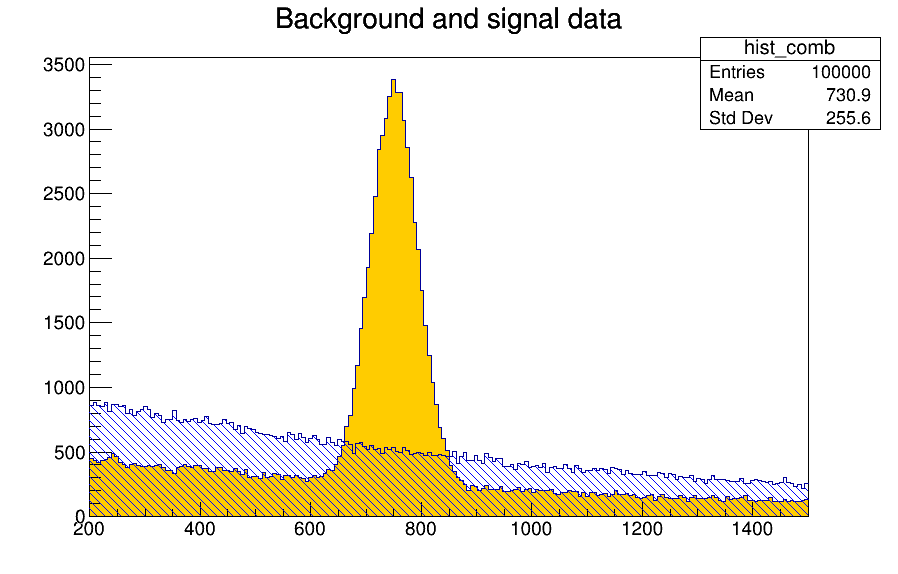
\includegraphics[width = 0.6\textwidth]{./exercise09_MCdata.png}
  \caption{Visualisation of datapoints for the \textit{background-only} (blue, dashed) and \textit{background+signal} (orange, filled) hypothesis.
  Each histogram contains \num{1e5} datapoints.}
  \label{fig:ex9_iter}
\end{figure}

\noindent Next, we calculate the test statistic $\Lambda$ for every iteration.
This is done via

\begin{equation}
\Lambda = \frac{\prod_{i=1}^{\num{e5}}f_{\textrm{sig}} + f_{\textrm{bkg}}}{\prod_{i=1}^{\num{e5}}f_{\textrm{bkg}}} = \prod_{i=1}^{\num{e5}}\frac{f_{\textrm{sig}} + f_{\textrm{bkg}}}{f_{\textrm{bkg}}}.
\label{eq:Lambda}
\end{equation}

\noindent Here is where we have some issues which we investigated but couldn't resolve.
An explanaition of our issue, which of course affects the rest of the exercise, is given below. \\

\noindent The second equality in equation \ref{eq:Lambda} is analytically correct but can give very different results numerically. \\
In our code we tested both parts of the equality.
Using the left part yields \texttt{-nan} while the right part yields \texttt{inf}.
This is due to the value of each parameter: \\
For values generated between \SI{200}{\giga\electronvolt} and \SI{1500}{\electronvolt} (same order as $a$) we can see that $f_{\textrm{bkg}}$ will be of the order of \num{e-3}.
Similar, for $f_\textrm{sig}$ we will get values of \num{e-2} at most.
When multiplying \num{e5} values which are all smaller than \num{1.0} we reach the storing limit very quickly.
In this example we already reach \num{e-100} after about \num{30} iterations\footnote{Obviously because $\prod_{1}^{100}$\num{e-3} $\approx$ \num{e-100}}.
Because of this we numerically divide by \num{0} yielding in a \texttt{nan} value. \\
The other case is more tricky.
Simply speaking, because of the positive contribution of $f_{\textrm{sig}}$ we expect to get a value larger than \num{1.0} on average.
Because we then multiply an averaged value larger than \num{1.0} \num{e5} times we reach an upper limit in storing numerical values yielding in \texttt{inf} as output. \\
In our script we tried both ways, so you can see the \texttt{-nan} and \texttt{inf} output by yourself.
To solve this issue one has to come up with a smarter way to calculate $\Lambda$ such that it does not diverge.
We were not able to find such method in time, so we leave it as it is.


\begin{comment}
\begin{figure}[H]
  \centering
  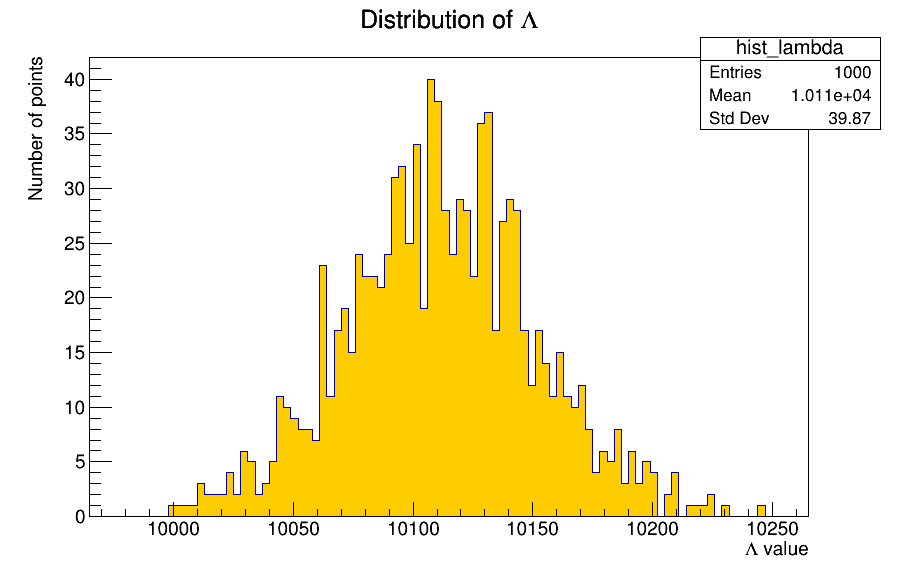
\includegraphics[width = 0.6\textwidth]{./exercise09_Lambda.png}
  \caption{Visualisation distribution of $\Lambda$.}
  \label{fig:ex9_lambda}
\end{figure}
\end{comment}

\end{myfont}
\end{document}
